\chapter{Conclusion and Outlook}
\label{Con}
\section{Conclusion}
\label{Con:Con}
During this master thesis the Routing Protocol for LLNs (RPL) has been studied. The study was based on the TOSSIM simulation of BLIP 2.0 with rfxlink radio stack. 
\newline

Low power consumption and low message overhead are crucial due to the resource constrains in LLNs. In RPL, the node which is closer to the root tend to have more control message traffic than the further ones. Furthermore, RPL uses Trickle algorithm to control the generating of DIOs. In various scenarios, it efficiently reduces the control message overhead as soon as the routing topology is stabilized.   
\newline

Objective Functions (OFs) are defined for RPL to meet different optimization objectives. OF0 and MRHOF are two OFs that are implemented in BLIP 2.0. The performances are evaluated in terms of RTT and packet loss with the application \texttt{UDPEcho}\@. The simulation results shows that OF0 only has good performance in simple and low density scenarios. For more dense scenarios, OF0 has unstable performances due to it chooses route without any objective guarantee. On the other hand, MRHOF with ETX routing metric has less packet loss and lower RTT than OF0 in larger and more complicated topologies, also the performance of MRHOF with ETX is more stable.  
\newline

\section{Outlook}
\label{outlook}
simulation with other scenarios can be conducted. Figure \ref{fig:container} shows a real life scenario. 
\begin{figure}[htbp]
  \begin{center}
    \leavevmode
      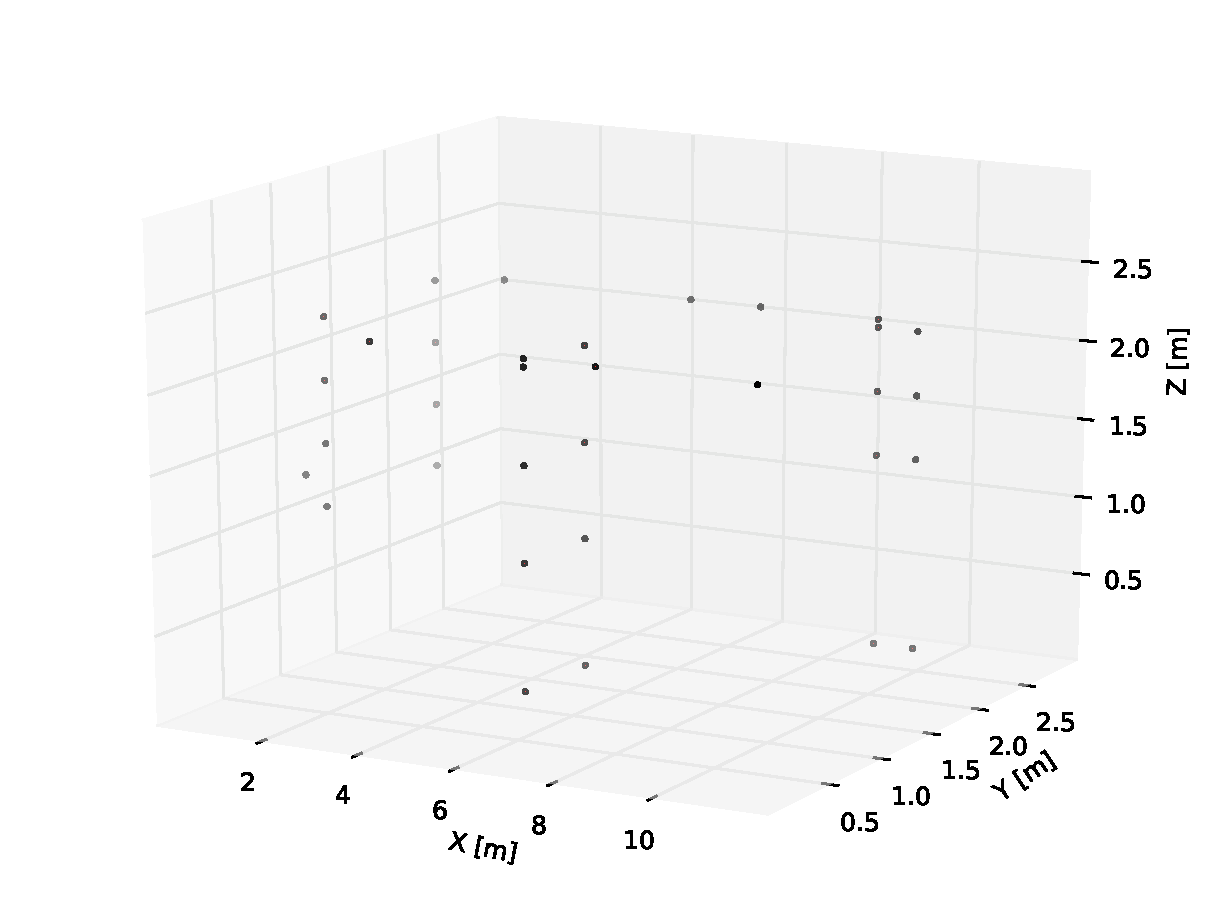
\includegraphics[scale=0.45]
      {/home/bo/Documents/Thesis/Final/Template/Pics/container.pdf}
   \caption{A container scenario: 32 sensor nodes and 1 border router, three types of connections depending on the position of the node: on top of the container, on top of the pallet, and in between the goods}
    \label{fig:container}
  \end{center}
\end{figure} 

Furthermore, many other applications can be simulated. In this thesis, the application UDPEcho shows the basic performances of RPL, but there are many other applications in BLIP 2.0 which are worth exploring, and the author
hopes they are done so in the near future.

